\pgfplotsset{width=\textwidth,compat=1.3}
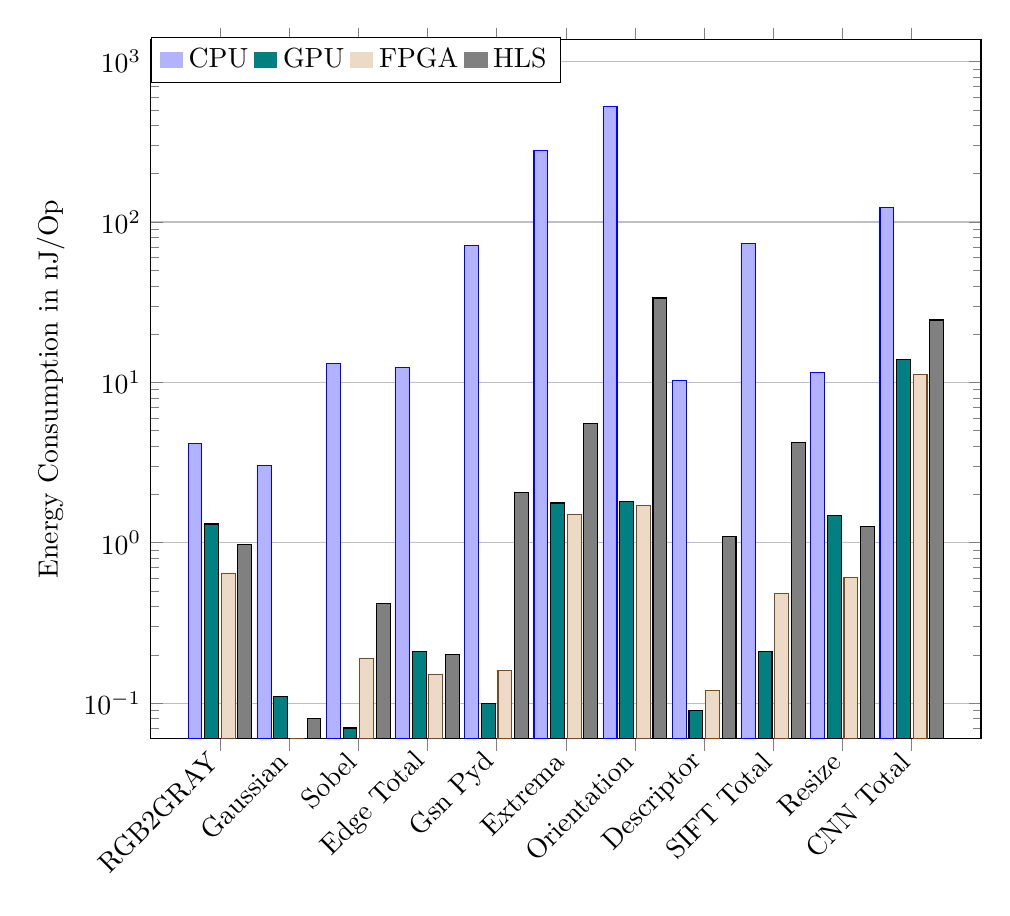
\begin{tikzpicture}
\begin{axis}[
    legend style={},
    ybar=1pt,
    bar width=5pt,
    ymin=0, % Set ymin to 1
    ymax=550,
    enlarge y limits={upper=0.15},
    ymode=log,
    legend image code/.code={\draw[#1, draw=none] (0cm,-0.1cm) rectangle (0.3cm,0.1cm);
                },
    ymajorgrids=true,
    legend style={at={(-0.00000009,0.971)},
                   anchor=west,legend columns=-2},
    ylabel={ Energy Consumption in nJ/Op},
    symbolic x coords={RGB2GRAY,Gaussian,Sobel,Edge Total,Gsn Pyd,Extrema,Orientation,Descriptor,SIFT Total,Resize,CNN Total},
    xtick=data,
    nodes near coords style={ anchor=west,rotate=90,inner xsep=0.5pt},
    x tick label style={ rotate=45, anchor=east},
    ]

\addplot coordinates {(RGB2GRAY,4.15) (Gaussian,3.03) (Sobel,13.04) (Edge Total,12.35) (Gsn Pyd,70.94) (Extrema,277.94) (Orientation,524.80) (Descriptor,10.22) (SIFT Total,73.27) (Resize,11.48) (CNN Total,123.50)};%CPU

\addplot [fill=teal!] coordinates {(RGB2GRAY,1.31) (Gaussian,0.11) (Sobel,0.07) (Edge Total,0.21) (Gsn Pyd,0.10) (Extrema,1.77) (Orientation,1.80) (Descriptor,0.09) (SIFT Total,0.21) (Resize,1.48) (CNN Total,13.96)};%GPU

\addplot coordinates {(RGB2GRAY,0.64) (Gaussian,0.06) (Sobel,0.19) (Edge Total,0.15) (Gsn Pyd,0.16) (Extrema,1.50) (Orientation,1.70) (Descriptor,0.12) (SIFT Total,0.48) (Resize,0.61) (CNN Total,11.17)};%FPGA

\addplot coordinates {(RGB2GRAY,0.98) (Gaussian,0.08) (Sobel,0.42) (Edge Total,0.20) (Gsn Pyd,2.06) (Extrema,5.57) (Orientation,33.60) (Descriptor,1.09) (SIFT Total,4.20) (Resize,1.27) (CNN Total,24.5)};%HLS

\legend{CPU,GPU,FPGA,HLS}
\end{axis}
\end{tikzpicture}
